\begin{figure}[H]
	\centering
	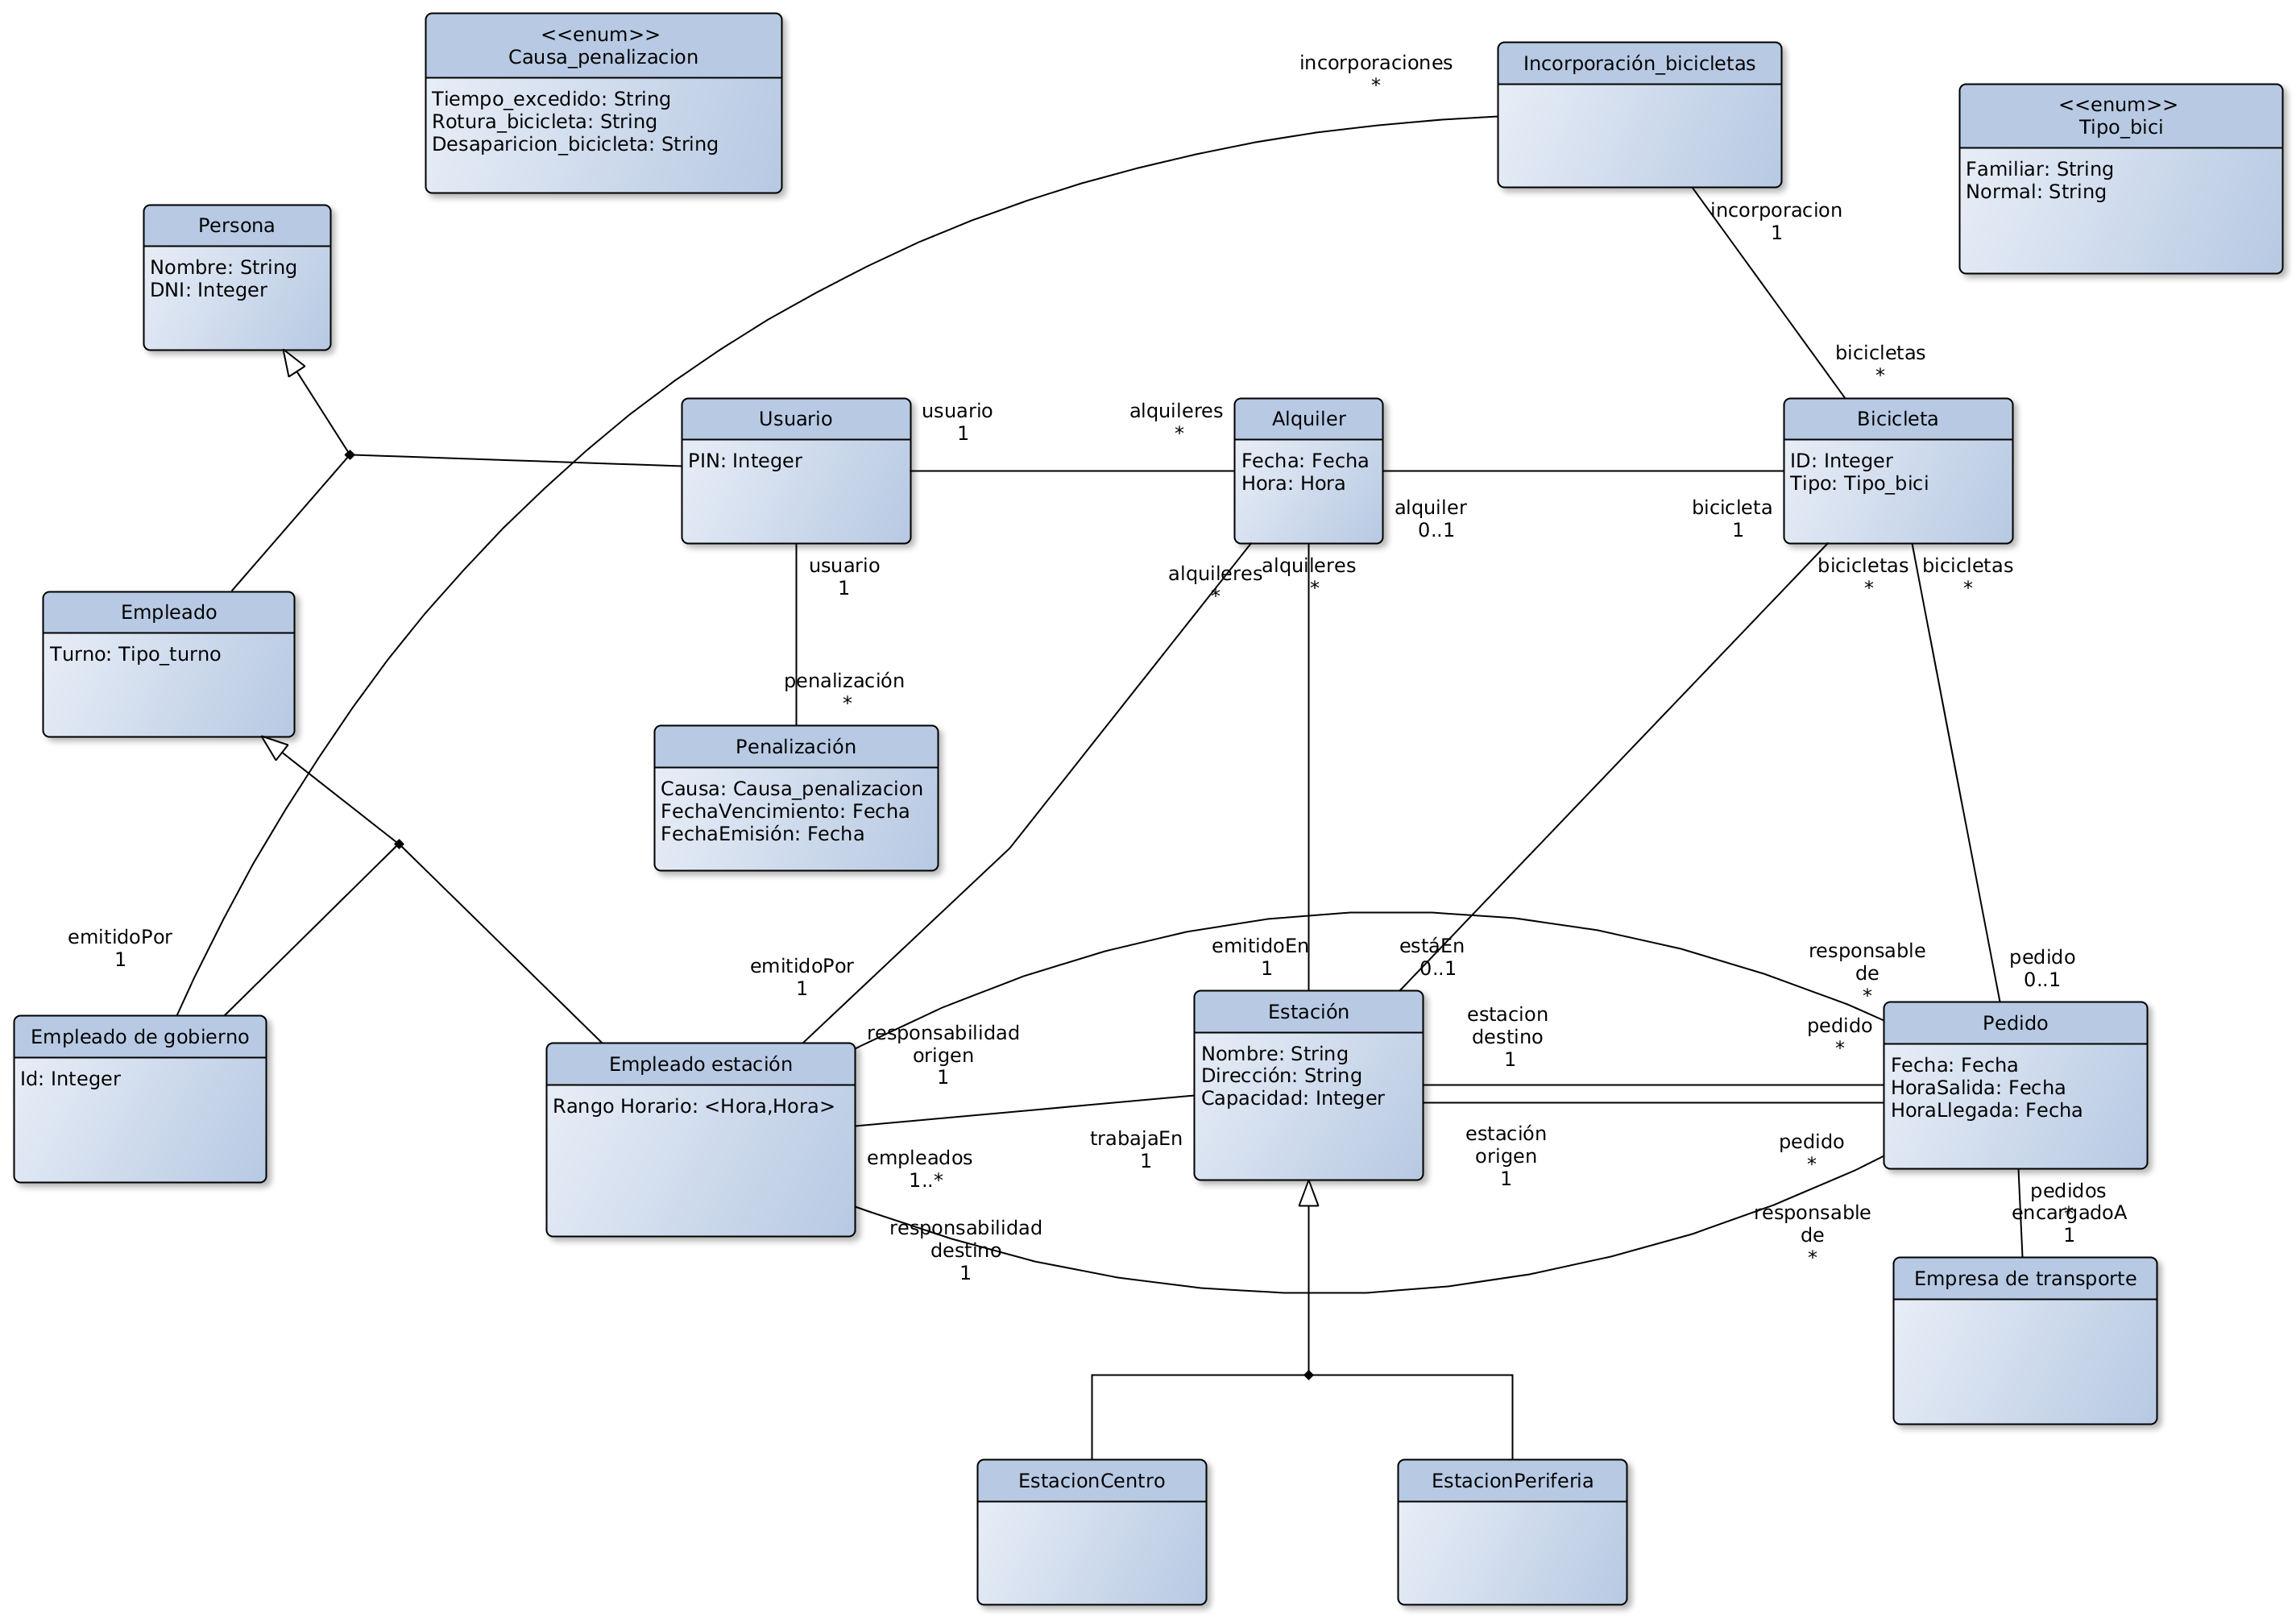
\includegraphics[scale=0.19]{imgs/diagrama_clases.png}
	\caption{Diagrama de Clases}
\end{figure}

\subsection{Invariantes en OCL}

\oclInv{Bicicleta}{Pedido.allInstances() $\rightarrow$ forAll(p1 | Pedido.allInstances() $\rightarrow$ forAll(p2 | p1.bicicletas $\rightarrow$ includes(self) $\wedge$ p2.bicicletas $\rightarrow$ includes(self) $\wedge$ p1$\neq$ p2 implies p1.horaSalida $\neq$ p2.horaSalida))}{No hay una bicicleta que esté en dos pedidos distintos para una misma hora}

~

\oclInv{Bicicleta}{(Bicicleta.allInstances() $\rightarrow$ select(b | b.id = self.id) $\rightarrow$ size() ) = 1}{Los identificadores de las bicicletas son distintos}

~

\oclInv{Usuario}{(Usuario.allInstances() $\rightarrow$ select(u | u.DNI = self.DNI) $\rightarrow$ size() ) = 1}{Los DNI's de los usuarios son distintos}

~


%CAMBIAR!!
%\oclInv{Usuario}{(self.penalizacion() $\rightarrow$ size() = 1) implies (
%(self.alquiler $\rightarrow$ size() = 1) implies ((self.alquiler.fecha \ < \ self.penalizacion().fechaEmision $\lor$
%self.alquiler.fecha \ > \ self.penalizacion.fechaVencimiento))))}{Si un usuario está penalizado, no puede alquilar bicicletas entre
%la fecha de origen de la penalización y la fecha de vencimiento}

~

\oclInv{Estacion}{(Estacion.allInstances() $\rightarrow$ select (e| e.nombre = self.nombre) $\rightarrow$ size() ) = 1}
{No hay estaciones con nombres iguales}

~

\oclInv{Estacion}{(Estacion.allInstances $\rightarrow$ select(e | e.direccion = self.direccion) -> size() ) = 1}
{No hay estaciones con direcciones iguales}
	
~

\oclInv{Pedido}{self.estacionOrigen $\neq$ self.estacionDestino}{No hay pedidos con una misma estación como origen y destino}

~

\oclInv{Pedido}{(self.bicicletas $\rightarrow$ size()) < self.estacionOrigen.capacidad}{La estación origen tiene suficiente capacidad como para albergar la cantidad de bicicletas a retirar requerida}

~

\oclInv{Pedido}{(self.bicicletas $\rightarrow$ size()) < self.estacionDestino.capacidad}{La estación destino tiene suficiente
capacidad para albergar la cantidad de bicicletas pedidas}

~

\oclInv{Pedido}{( (self.bicicletas $\rightarrow$ forAll(b | ((b.alquiler $\rightarrow$ size() = 1) implies
(b.alquiler.Hora $\neq$ self.HoraSalida))))) }{Solo se pueden transportar bicicletas que no estén alquiladas}

~

\oclInv{EmpleadoEstacion}{(Estacion.allInstances() $\rightarrow$ select ( e | e.id = self.id )) 
$\rightarrow$ size()) = 1 }{No puede haber empleados de estación iguales que trabajen en estaciones distintas}

~

\oclInv{EstacionCentro}{(EstacionPerifera.allInstances()) $\rightarrow$ forAll(e | e.capacidad*2 $\leq$ self.capacidad)}{
Las estaciones del centro tienen más capacidad que las de la periferia. (La proporción del doble parece una aproximación
razonable)}

~

\oclInv{Alquiler}{((self.emitidoEn.empleados $\rightarrow$ select(e | e.id = self.emitidoPor.id)) $\rightarrow$ size()) = 1}{Los alquileres tienen que ser emitidos por algún empleado que trabaje en la estación en donde fue hecho}

~

\oclInv{Pedido}{((self.EstacionDestino.empleados $\rightarrow$ select(e | e.id = self.responsabilidadDestino.id)) $\rightarrow$ size()) = \ 1}{Los pedidos tienen que tener como responsable destino a un empleado que trabaje en la estacion destino}
~


\oclInv{Pedido}{((self.EstacionOrigen.empleados $\rightarrow$ select(e | e.id = self.responsabilidadOrigen.id)) $\rightarrow$ size()) = \ 1}{Los pedidos tienen que tener como responsable origen a un empleado que trabaje en la estacion origen}

%\oclInv{Incorporación\_bicicletas}{(self.bicicletas $\rightarrow$ size()) < \ self.estacionDestino.capacidad}{La estación destino debe tener suficiente capacidad como para albergar la cantidad de bicicletas a incorporar}

~

\oclInv{Bicicleta}{Bicicleta.AllInstances() $\rightarrow$ forAll(b | (b.alquiler $\rightarrow$ size() = 1) implies (b.EstaEn $\rightarrow$ size() = 0)) }{Si una bicicleta está alquilada entonces no se encuentra en ninguna estación}

~

%%CHEQUEAR

\oclInv{Usuario}{self.penalizaciones $\rightarrow$ forAll(p | self.alquileres $\rightarrow$ forAll(a | a.fecha < \ p.fechaEmision $\lor$ a.fecha > \ p.fechaVencimiento))}{Ningún usuario puede tener un alquiler cuya fecha coincida con el plazo de alguna penalización}

%%
~

\oclInv{Estacion}{self.capacidad $\geq$ self.bicicletas $\rightarrow$ size()}{La capacidad de una estación nunca es superada por la cantidad de bicicletas presentes}

%Faltan:

\oclInv{}{}{Si una bicicleta desaparece no aparecerá en ningún pedido o alquiler futuro}
\oclInv{}{}{Los empleados que tienen responsabilidad sobre un pedido deben estar en sus puestos de trabajo al momento de ser asignado}
\oclInv{}{}{Un usuario no puede tener alquileres solapados}



%Otras para agregar:
%\begin{itemize}
%\item No puede haber una bicicleta alquilada que este en una estacion (listo)
%\item No se puede superar la capacidad de la estacion al incorporar nuevas bicicletas. (listo)
%\item El pedido tiene que tener como responsable a un empleado que trabaje en la estacion destino. (listo)
%\item El alquiler tiene que ser emitido por un empleado que trabaje en la estación en donde fue hecho. (listo)
%\item No se solapan alquileres y penalizaciones. (listo)
%\item Hay una penalizacion si y solo si hay un alquiler indebido.
%\item La capacidad nunca es superada por la cantidad de bicicletas presentes (listo)
%\end{itemize}

\subsection{Algunas aclaraciones sobre las relaciones}

\begin{itemize}
	\item Planteamos la relación 'emitidoPor' entre las clases Alquiler y Empleado de estación para tener en claro quién es el responsable por cada alquiler que se realiza en las distintas estaciones y de esta forma evitar posibles irregularidades en el servicio.
	\item Por el mismo motivo, planteamos las relaciones 'responsabilidad origen' y 'responsabilidad destino' entre las clases Pedido y Empleado de estación. Cuando el sistema emite un pedido de movilización de bicicletas, un empleado de la estación destino se encarga de modificar el stock de dicha estación en base al pedido realizado. Lo mismo sucede en la estación origen.
	\item Planteamos la relación 'emitidoPor' entre las clases Empleado de gobierno e Incorporacion\_bicicletas puesto que queremos evitar posibles errores en la cantidad de bicicletas ingresadas, teniendo así un responsable para cuestionar y sancionar severamente. Al momento de incorporar nuevas bicicletas, el sistema las distribuye según las necesidades actuales de la Red de Ciclovías. 
\end{itemize}




